%-------------------------
% Matteo Dante - Curriculum Vitae (IT)
% Template: Harshibar (MIT) - adattato
%-------------------------

\documentclass[a4paper,10pt]{article}

\usepackage{latexsym}
\usepackage[empty]{fullpage}
\usepackage{titlesec}
\usepackage{marvosym}
\usepackage[usenames,dvipsnames]{color}
\usepackage{verbatim}
\usepackage{enumitem}
\usepackage[hidelinks]{hyperref}
\usepackage{fancyhdr}
\usepackage[italian]{babel}
\usepackage{tabularx}
\usepackage{graphicx}


\definecolor{light-grey}{gray}{0.83}
\definecolor{dark-grey}{gray}{0.3}
\definecolor{text-grey}{gray}{.08}

\DeclareRobustCommand{\ebseries}{\fontseries{eb}\selectfont}
\DeclareTextFontCommand{\texteb}{\ebseries}

\usepackage{contour}
\usepackage[normalem]{ulem}
\renewcommand{\ULdepth}{1.8pt}
\contourlength{0.8pt}
\newcommand{\myuline}[1]{%
  \uline{\phantom{#1}}%
  \llap{\contour{white}{#1}}%
}

\usepackage{tgheros}
\renewcommand*\familydefault{\sfdefault}
\usepackage[T1]{fontenc}

\graphicspath{{../images/}}

\pagestyle{fancy}
\fancyhf{}
\fancyfoot{}
\renewcommand{\headrulewidth}{0pt}
\renewcommand{\footrulewidth}{0pt}

\addtolength{\oddsidemargin}{-0.7in}
\addtolength{\evensidemargin}{0in}
\addtolength{\textwidth}{1.4in}
\addtolength{\topmargin}{-1.2in}
\addtolength{\textheight}{2.3in}
\setlength{\footskip}{4pt}

\urlstyle{same}

\raggedbottom
\raggedright
\setlength{\tabcolsep}{0in}

\titleformat{\section}{
    \bfseries \raggedright \large
}{}{0em}{}[\color{light-grey}{\titlerule[2pt]} \vspace{-4pt}]
\titlespacing*{\section}{0pt}{8pt}{6pt}

\newcommand{\resumeItem}[1]{
  \item\small{
    {#1 \vspace{-1pt}}
  }
}

\newcommand{\resumeSubheading}[4]{
  \vspace{-1pt}\item
    \begin{tabular*}{\textwidth}[t]{l@{\extracolsep{\fill}}r}
      \textbf{#1} & {\color{dark-grey}\small #2}\vspace{1pt}\\
      \textit{#3} & {\color{dark-grey} \small #4}\\
    \end{tabular*}\vspace{-4pt}
}

\newcommand{\resumeProjectHeading}[3]{%
    \item\small
    \textbf{#1}\hfill{\color{dark-grey}\small #3}\par
    \vspace{1pt}\small #2\par\vspace{2pt}
}

\renewcommand\labelitemii{$\vcenter{\hbox{\tiny$\bullet$}}$}

\newcommand{\resumeSubHeadingListStart}{\begin{itemize}[leftmargin=0in, label={}]}
\newcommand{\resumeSubHeadingListEnd}{\end{itemize}}
\newcommand{\resumeItemListStart}{\begin{itemize}}
\newcommand{\resumeItemListEnd}{\end{itemize}\vspace{0pt}}

\color{text-grey}

\begin{document}

%----------HEADER----------
\begin{minipage}[c]{0.20\textwidth}
  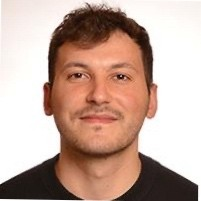
\includegraphics[width=\linewidth]{profile-pic.jpeg}
\end{minipage}\hfill
\begin{minipage}[c]{0.78\textwidth}
  \raggedright
  {\Huge \textbf{Matteo Dante}}\\[4pt]
  {\large Senior Software Engineer \textperiodcentered{} Full-Stack \& Backend}\\[6pt]
  \small
  \Email\ \href{mailto:matteo.dante659@gmail.com}{\texttt{matteo.dante659@gmail.com}} \hspace{4pt}$|$\hspace{4pt}
  \Mundus\ \href{https://matteodante.it}{\myuline{matteodante.it}}\\
  GitHub: \href{https://github.com/matteodante}{\myuline{matteodante}} \hspace{4pt}$|$\hspace{4pt}
  LinkedIn: \href{https://linkedin.com/in/matteo-dante-3705b5164}{\myuline{matteo-dante}} \hspace{4pt}$|$\hspace{4pt}
  Svizzera, Permesso G
\end{minipage}

\vspace{8pt}

%-----------PROFILO-----------
\section{PROFILO}
\small
Senior software engineer, 8+ anni su sistemi in produzione per aviazione, piattaforme consumer ad alto traffico e retail. Attualmente tra i principali ingegneri di una piattaforma greenfield per l'addestramento piloti in Pilatus Aircraft, rilasciata on-premise sulle basi delle forze aeree. Appassionato di programmazione fin da bambino, ma interessato anche a finanza e mercati azionari, filosofia, moto e palestra.

%-----------ESPERIENZA-----------
\section{ESPERIENZA}
  \resumeSubHeadingListStart

    \resumeSubheading
      {Pilatus Aircraft Ltd}{04/2024 -- Presente}
      {Senior Full-Stack Software Engineer (principalmente frontend)}{Stans (2024--25), Chiasso (2025+), Svizzera}
      \resumeItemListStart
        \resumeItem{\textbf{Piattaforma greenfield per l'addestramento piloti} rilasciata \textbf{on-premise su basi delle forze aeree svizzere ed estere}, sotto standard dell'industria della difesa. Team di 10 (6 FE, 4 BE).}
        \resumeItem{\textbf{Frontend piattaforma}: costruzione su architettura \textbf{microfrontend}. Pipeline di build/deploy isolate per consegna indipendente di ogni sistema in ambienti air-gapped.}
        \resumeItem{\textbf{Design system}: cura del DS usato dal team frontend di 6 ingegneri. Primary reviewer del codice frontend. Conduzione colloqui di selezione e onboarding dei nuovi ingegneri.}
      \resumeItemListEnd

    \resumeSubheading
      {DonTouch SA}{07/2023 -- 04/2024}
      {Backend Engineer}{Chiasso, Svizzera}
      \resumeItemListStart
        \resumeItem{Piattaforma consumer (tier di abbonamento, recensioni, algoritmo di rating) con \textbf{2M+ utenti registrati, 10k+ concorrenti al picco}. Team di 5 BE e 6 FE. Architettura a microservizi backend.}
        \resumeItem{\textbf{Backend app mobile advertiser}: abbonamenti geografici, sospensione/ripresa, pagamenti.}
      \resumeItemListEnd

    \resumeSubheading
      {Hexa Credit Care}{11/2019 -- 07/2023}
      {Full-Stack Developer}{Roma, Italia}
      \resumeItemListStart
        \resumeItem{CRM multi-tenant e sales analytics per \textbf{300 operatori di call center} tra recupero crediti e vendite B2C. Clienti enterprise: \textbf{Fastweb, Sorgenia}. Progressione \textbf{da junior a senior} in tre anni.}
        \resumeItem{\textbf{Architettura multi-tenant}: isolamento di configurazione e dati per cliente su un unico codebase.}
        \resumeItem{\textbf{Reporting real-time}: layer che alimenta le dashboard di operatori e manager.}
      \resumeItemListEnd

    \resumeSubheading
      {Galileo SpA}{03/2018 -- 11/2019}
      {Full-Stack Developer}{Roma, Italia}
      \resumeItemListStart
        \resumeItem{Piattaforma aziendale per catalogo, media e logistica di un retailer con \textbf{60+ negozi fisici e 40.000+ SKU}.}
        \resumeItem{\textbf{Integrazione IBM AS/400}: interrogazione del database dalla piattaforma web.}
        \resumeItem{\textbf{Catalogo B2B e pipeline PDF/print}, libreria di asset multimediali, tooling barcode/SKU per il magazzino.}
      \resumeItemListEnd

  \resumeSubHeadingListEnd

%-----------PROGETTI-----------
\section{PROGETTI}
    \resumeSubHeadingListStart

      \resumeProjectHeading
        {GymTree}
        {\textit{Progetto personale, sviluppato in autonomia.} Piattaforma fitness: API backend, web coach, app mobile trainee, worker background. \textbf{AI in produzione} per chat persistente col coach e programmi personalizzati di allenamento e nutrizione.}
        {2025}

      \resumeProjectHeading
        {\href{https://github.com/matteodante/claude-local-docs}{claude-local-docs}}
        {\textit{Progetto personale, sviluppato in autonomia.} Plugin open source per Claude Code. Indicizzatore di documentazione local-first con \textbf{vector embeddings, BM25, Reciprocal Rank Fusion, cross-encoder reranking}.}
        {}

      \resumeProjectHeading
        {\href{https://matteodante.it}{matteodante.it}}
        {\textit{Progetto personale, sviluppato in autonomia.} Portfolio 3D interattivo con assistente AI in streaming. Next.js 16, React Three Fiber, OpenAI Responses API in streaming, i18n EN/IT.}
        {}

    \resumeSubHeadingListEnd

%-----------FORMAZIONE-----------
\section{FORMAZIONE}
  \resumeSubHeadingListStart
    \resumeSubheading
      {Università Telematica Unitelma Sapienza}{09/2018 -- 2021}
      {Laurea in Informatica \textit{(non completata)}}{Roma, Italia}
    \resumeSubheading
      {Istituto E. Fermi}{09/2012 -- 07/2017}
      {Diploma in Sistemi Informativi Aziendali}{Italia}
  \resumeSubHeadingListEnd

%-----------COMPETENZE-----------
\section{COMPETENZE}
 \begin{itemize}[leftmargin=0in, label={}]
    \small{\item{
     \textbf{Linguaggi \& Runtime}: TypeScript, Node.js, PHP, .NET, Java\vspace{2pt}\\
     \textbf{Frontend \& Mobile}: React 19, Next.js App Router, React Native (Expo), microfrontend con Module Federation, React Three Fiber, Tailwind\vspace{2pt}\\
     \textbf{Backend \& Dati}: Laravel, Hono, Express, tRPC, REST; PostgreSQL, MySQL, MS SQL Server, Redis, Prisma; BullMQ\vspace{2pt}\\
     \textbf{AI \& Search}: API OpenAI/Anthropic; agenti LLM, structured output, streaming; RAG con embeddings, BM25, RRF, cross-encoder reranking\vspace{2pt}\\
     \textbf{Infra \& Qualità}: Docker, Turborepo, Vercel, Railway; deployment on-premise / air-gapped; Vitest, Sentry; OWASP, OAuth/JWT; tooling AI dev: Claude Code, Cursor
    }}
 \end{itemize}

\end{document}
